\documentclass{beamer}
\usepackage[utf8]{inputenc}
\usepackage{color}
\usepackage{isomath}
\usepackage{amsmath}
\usepackage{amsfonts}
\usepackage{gnuplottex}
\usepackage{graphicx}


\title{Dynamic loading of 3D models}
\subtitle{Computing Project - PROJ-H-402}
\author{Tim Lenertz}
\institute{ULB, MA1 INFO}
\date{\today}

\usetheme{Antibes}
\usecolortheme{whale}

\begin{document}

\begin{frame}
	\titlepage
\end{frame}

\begin{frame}{Contents}
	\tableofcontents
\end{frame}

\section{Introduction}

\begin{frame}{Introduction}
	\begin{itemize}
	\item Large XYZRGB point clouds
	\item Composite point clouds
	\item High density 3D scanner
	\item $\Rightarrow$ Too many points to process as whole
	\item \textbf{Goal}: Dynamically extract smaller sets for visualization
	\item Filtering techniques
	\item Data structure and file format
	\end{itemize}
\end{frame}

\begin{frame}{Example}
	\begin{columns}[t|t]
	\column[t]{.5\textwidth}
		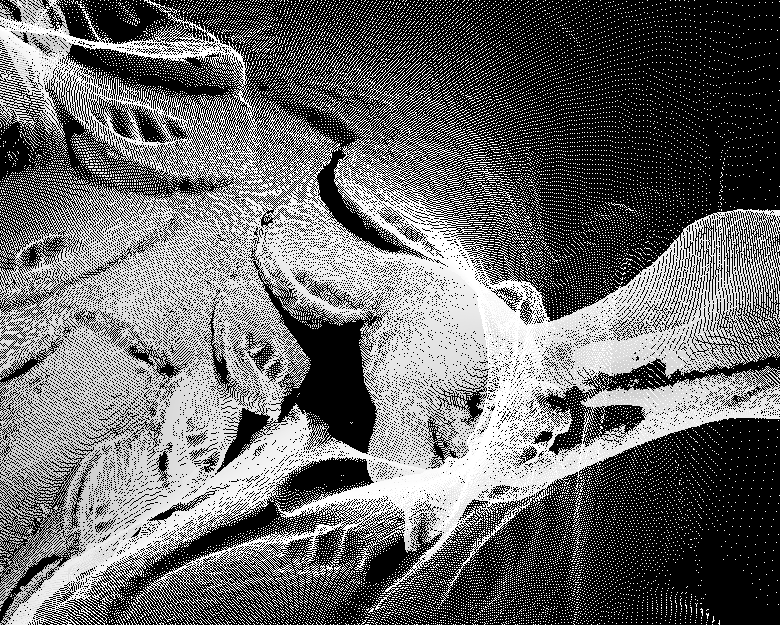
\includegraphics[width=\textwidth]{dir.png} \\
		Unfiltered render \\
		$\Rightarrow$ buffer overflow
	\column[t]{.5\textwidth}
		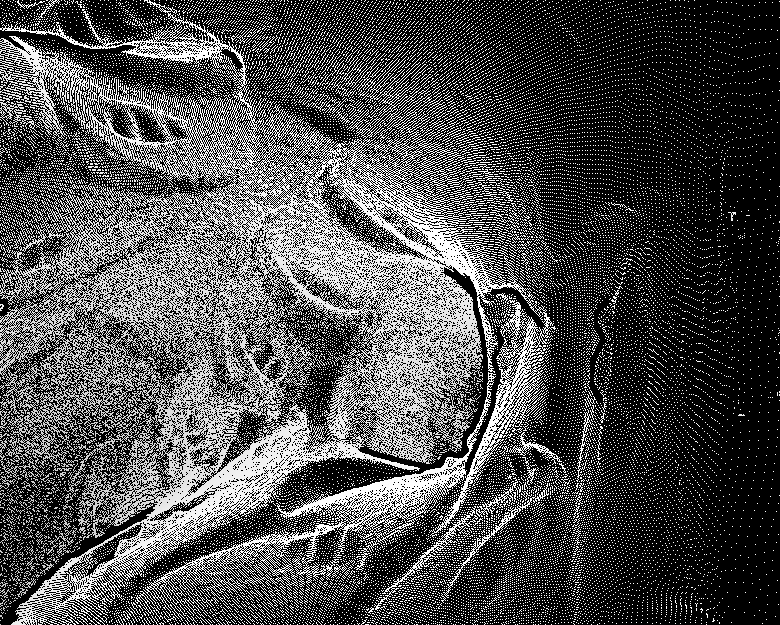
\includegraphics[width=\textwidth]{str.png} \\
		Using Octree structure \\
		8 downsampled LOD regions
	\end{columns}
\end{frame}

\begin{frame}{Application Screenshot}
	\begin{center}
	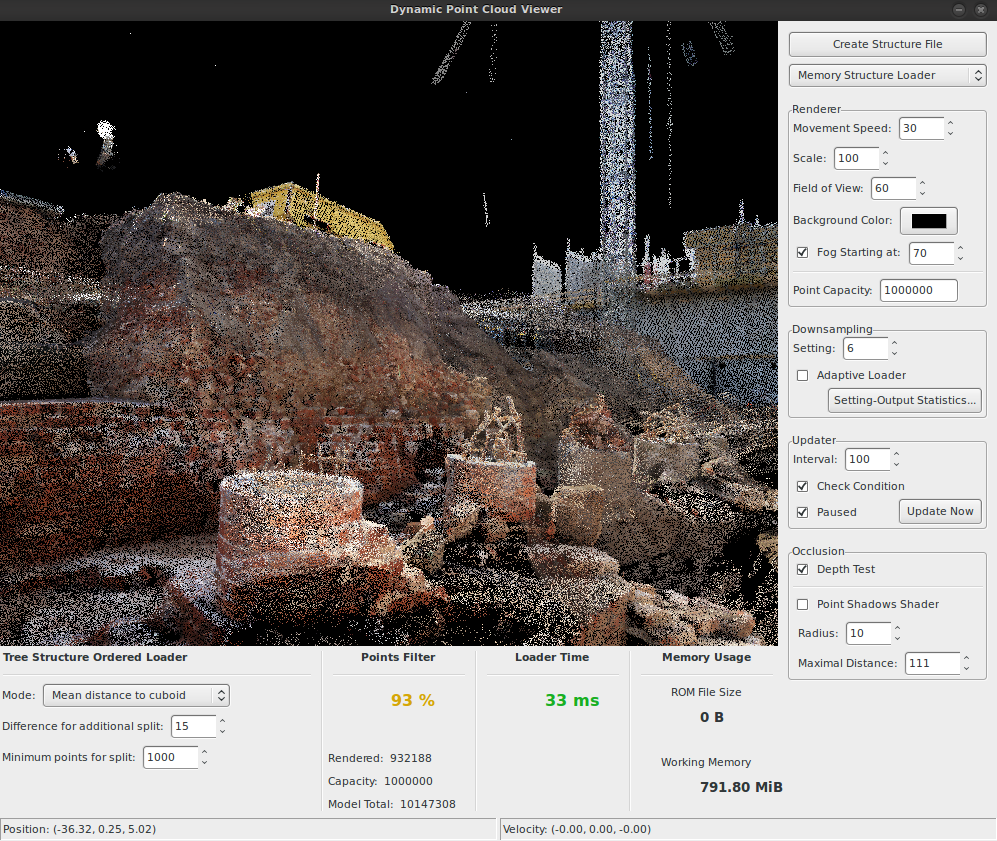
\includegraphics[width=.8\textwidth]{screenshot.png}
	\end{center}
\end{frame}

\section{Filtering}

\begin{frame}{Mechanism}
	\begin{itemize}
	\item Extract part $P'$ of model $P$
	\item Relative to current camera position, orientation, etc.
	\item $P'$ filtered to remove unnecessary parts
	\item $\rightarrow$ Fit into renderer capacity $C$
	\item $\rightarrow$ Retain visual quality
	\item Implemented using underlying \emph{data structure}
	\item Data structure created in preprocessing step
	\item Extraction of $P'$  is time critical
	\end{itemize}
\end{frame}

\begin{frame}{Techniques}
	\begin{itemize}
	\item Theoretical description of $f_{P}$
	\item Without regard for data structure
	\item Techniques used:
		\begin{description}
		\item[View frustum culling] Render only visible parts of model
		\item[Downsampling] Reduce point density in distant regions
		\item[Occlusion culling] Don't render hidden surfaces
		\end{description}
	\end{itemize}
\end{frame}

\subsection{View frustum culling}

\begin{frame}{Frustum culling}
	\begin{columns}[c]
	\begin{column}[T]{.6\textwidth}
		\begin{itemize}
		\item Remove invisible points
		\item Most effective part
		\item Often removes $\geq 1/2$
		\item With data structure: Remove entire regions
		\item $\rightarrow$ Before sending to GPU
		\end{itemize}
	\end{column}
	\begin{column}[T]{.4\textwidth}
		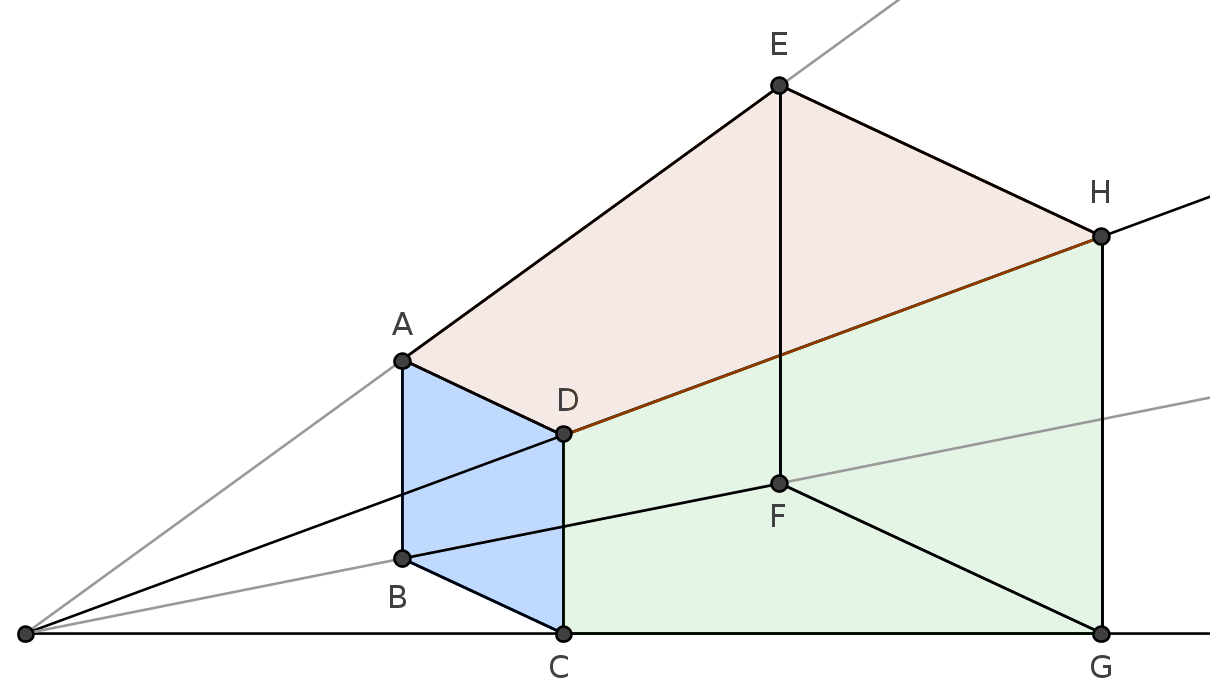
\includegraphics[width=4cm]{frustum.png}
	\end{column}
	\end{columns}
\end{frame}

\begin{frame}{Frustum}
	\begin{columns}[c]
	\begin{column}[T]{.6\textwidth}
		\begin{itemize}
		\item Frustum = 6 planes \\
		(near, far, top, bottom, left, right)
		\item Apex = camera
		\item Entirely defined by 4x4 projection matrix $\matrixsym{M}$
		\item $\matrixsym{M} = \matrixsym{P} \times \matrixsym{V}$
		\item $\matrixsym{V}$ = view matrix \\
		camera position and orientation
		\item $\matrixsym{P}$ = projection matrix \\
		perspective or parallel 3D to 2D projection
		\end{itemize}
	\end{column}
	\begin{column}[T]{.4\textwidth}
		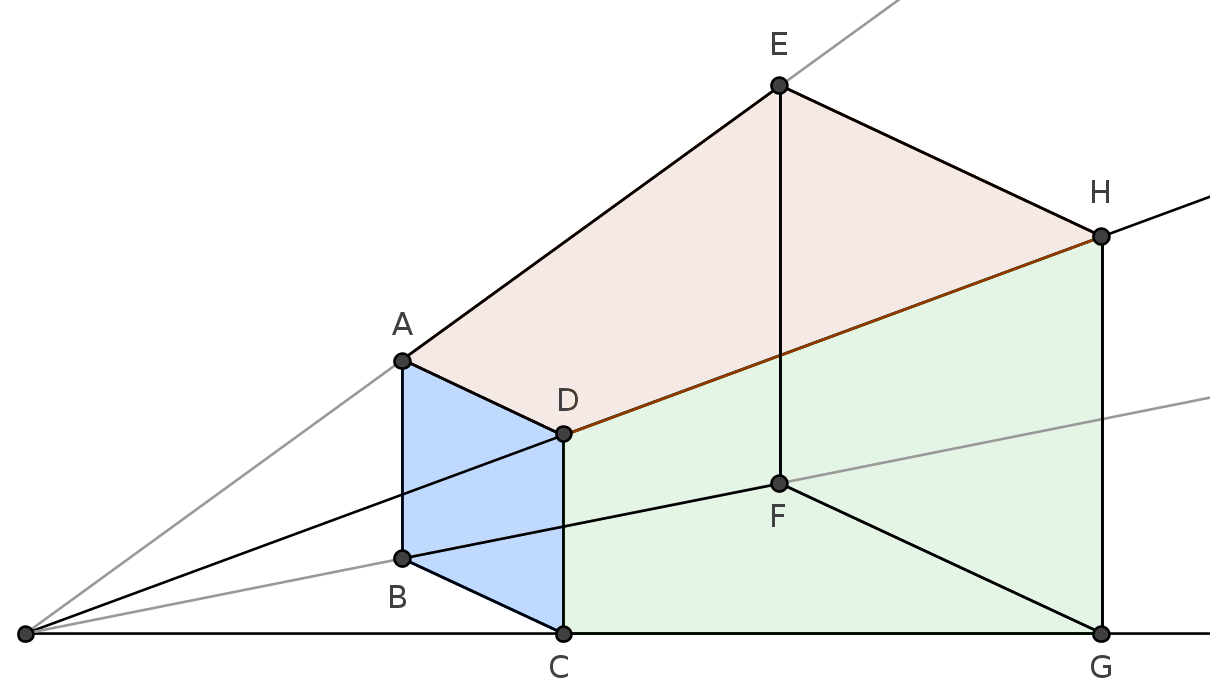
\includegraphics[width=4cm]{frustum.png}
	\end{column}
	\end{columns}
\end{frame}


\begin{frame}{Projection matrix}
	\begin{itemize}
	\item Using \emph{homogeneous coordinates}
	\item For 4x4 matrices
	\item Vector $[x, y, z, w] \rightarrow [\frac{x}{w}, \frac{y}{w}, \frac{z}{w}]$
	\item $w = 0$: direction \quad \quad $w = 1$: position
	\item Non-linear: Division by $w$
	\item Allows for perspective foreshortening
	\item Perspective projection matrix:
	\end{itemize}
	\begin{displaymath}
	\matrixsym{P} = \begin{bmatrix}
	\frac{f}{w/h} & 0 & 0 & 0 \\
	0 & f & 0 & 0 \\
	0 & 0 & \frac{z_{\mathrm{far}} + z_{\mathrm{near}}}{z_{\mathrm{near}} - z_{\mathrm{far}}} & \frac{2 \times z_{\mathrm{far}} \times z_{\mathrm{near}}}{z_{\mathrm{near}} - z_{\mathrm{far}}} \\
	0 & 0 & -1 & 0
	\end{bmatrix}
	\text{ with }
	f = \frac{1}{\tan(\frac{\lambda}{2})}
	\end{displaymath}
\end{frame}


\subsection{Downsampling}

\begin{frame}{Downsampling}
	\begin{itemize}
	\item Reduce point density
	\item Foreshortening $\rightarrow$ downsample distant parts
	\item Points are always located on (unknown) surfaces
	\item Density = $n/A$, locally constant, but can vary in composite models
	\item Downsampling ratio: $r(d) \in [0,1]$
	\item $d$ = distance to camera (of data structure region)
	\item Variants:
		\begin{itemize}
		\item Weighted points
		\item LOD (level of detail) regions
		\end{itemize}
	\end{itemize}
\end{frame}

\subsubsection{Weighted points}

\begin{frame}{Weighted points}
	\begin{itemize}
	\item Assign weight $w \in [0,1]$ to each point
	\item Downsampled points = subset \\
	$P' = \{ p \in P : w(p) < r(d(p)) \}$
	\item $w$ need to be uniformly distributed among points
	\item $\rightarrow$ Associate random weights 
	\item $r(d)$ can take any value
	\item $\rightarrow$ Visual continuity
	\item Random $\rightarrow$ Irregular pattern
	\end{itemize}
\end{frame}

\begin{frame}{Weighted points (2)}
	\begin{center}
	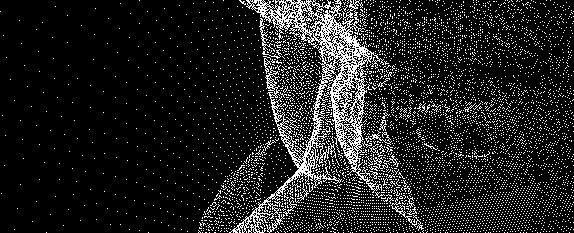
\includegraphics[width=.9\textwidth]{random_weights.png} \\
	Random weights $\Rightarrow$ irregular pattern
	\end{center}
\end{frame}

\subsubsection{LOD regions}

\begin{frame}{LOD regions}
	\begin{itemize}
	\item Precompute downsampled point sets
	\item Usually 4, 8 or 16
	\item Fixed $r$
	\item No time constraint for downsampling
	\item Visual discontinuitites
	\end{itemize}
\end{frame}

\begin{frame}{LOD regions (2)}
	\begin{center}
	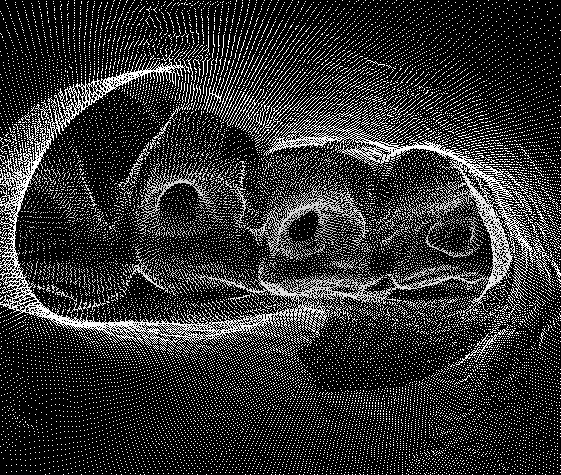
\includegraphics[width=.7\textwidth]{uniform_example.png} \\
	Uniform downsampling
	\end{center}
\end{frame}

\subsubsection{Uniform downsampling}

\begin{frame}{LOD regions}
	\begin{itemize}
	\item Algorithm to get more regular pattern
	\item Constant $r$
	\item Cubes grid with side length $l$
	\item Take only mean point
	\item Find $l$ for expected $r$: Dichotomic search
	\end{itemize}
	\begin{center}
	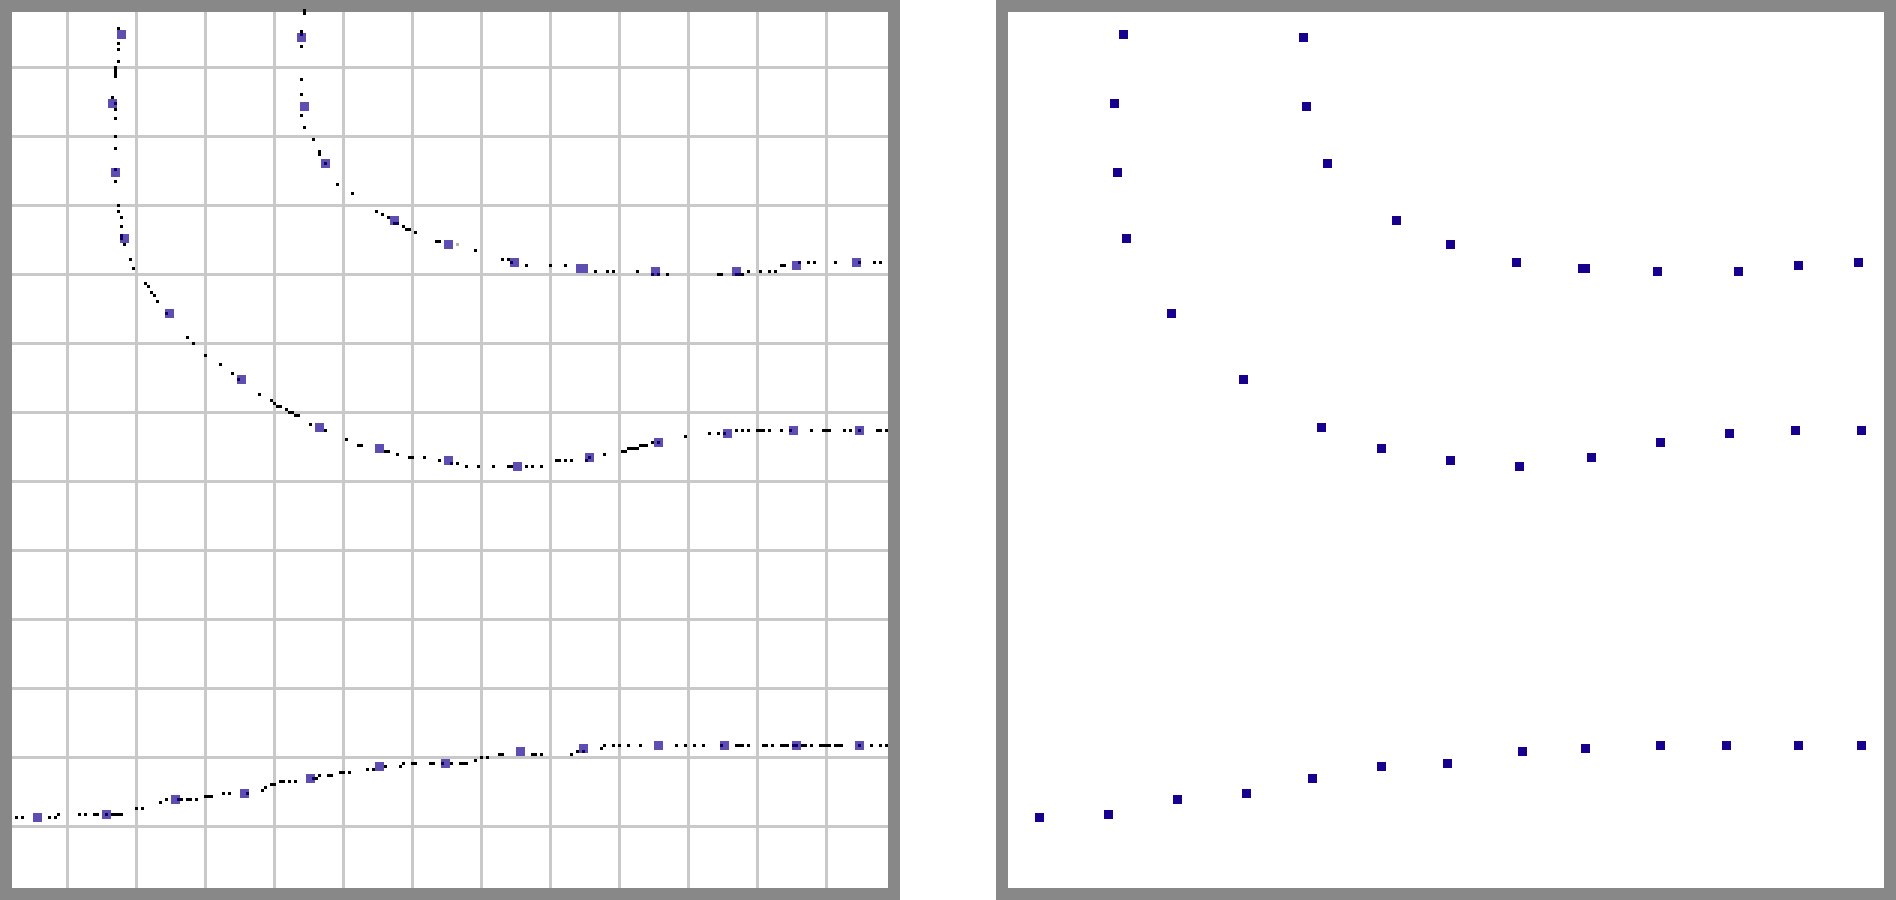
\includegraphics[width=.8\textwidth]{uniform.png}
	\end{center}
\end{frame}

\begin{frame}{LOD regions (2)}
	Cubes side length $l$ VS output number of points $n$ \\
	\resizebox{!}{0.6\textwidth}{\begin{gnuplot}
	set terminal epslatex color
	set xlabel "$l$"
	set ylabel "$n / |P|$"
	plot \
		"stat\_dragon.dat" using 1:($2/3609599+0*$2) smooth unique linetype rgb "black" title "dragon.ply", \
		"stat\_statuette.dat" using 1:($2/4999995+0*$2) smooth unique linetype rgb "red" title "statuette.ply", \
		"stat\_scan.dat" using 1:($2/681124+0*$2) smooth unique linetype rgb "blue" title "scan.ply"
\end{gnuplot}
}
\end{frame}


\begin{frame}{LOD regions (3)}
	Not fully monotonic. Close-up: \\
	\resizebox{!}{0.6\textwidth}{\begin{gnuplot}
	unset key
	set ylabel "$n$"
	set xlabel "$s$"
	plot "uniform\_stat\_detail.dat" smooth unique
\end{gnuplot}
}
\end{frame}

\subsubsection{Downsampling ratio choice}

\begin{frame}{Downsampling ratio choice}
	\begin{itemize}
	\item Definition of $r(d)$
	\item Decreasing with $d$
	\item Distance $\rightarrow$ Level $\rightarrow$ Ratio
	\item For \emph{LOD regions}: $L$ possible levels
	\item For \emph{weighted points}: Level can be continuous
	\end{itemize}
\end{frame}

\begin{frame}{Downsampling level}
	Downsampling level $\ell(d, s)$: \\
	\begin{displaymath}
		\ell(d, s) = \begin{cases}
			\min \{ \frac{d - d_{0}}{\Delta d}, L-1 \} & d > d_{0} \\
			0 & d \leq d_{0} \vee s = 0
		\end{cases}
	\end{displaymath}
	\begin{columns}[c]
		\begin{column}[T]{.7\textwidth}
			\resizebox{!}{.65\textwidth}{\begin{gnuplot}
	set terminal epslatex color
	set ylabel "level"
	set xlabel "$d$"
	set ytics (0, 1, 2, 3, 4, 5, 6, 7, 8, 9, 10, 11, 12, 13, 14, 15)

	levels = 16
	xp = 1.3
	maxd = 700

	set xrange [0:maxd]
	set yrange [0:levels + 3]
	unset autoscale

	start_distance(b) = b**xp
	step_distance(b) = b
	constrain_lvl(l) = (l > levels - 1) ? (levels - 1) : l
	b(s) = 250 / s

	l(d, s) = constrain_lvl( \
		(d > start_distance(b(s))) ? ((d - start_distance(b(s))) / step_distance(b(s))) : 0 \
	)
	
	plot [d=0:maxd] \
		floor(l(d, 20)) with steps lt rgb "black" title "$s = 20$", \
		floor(l(d, 10)) with steps lt rgb "blue" title "$s = 10$", \
		floor(l(d, 50)) with steps lt rgb "red" title "$s = 50$"
\end{gnuplot}
}
		\end{column}
		\begin{column}[T]{.3\textwidth}
			$L$ = nb of levels \\
			$s$ = setting \\
			$b = \frac{250}{s}$ \\
			$\Delta d = b$ \\
			$d_{0} = b^{1.3}$
		\end{column}
	\end{columns}
\end{frame}


\begin{frame}{Downsampling ratio}
	Downsampling ratio $r(\ell)$ for level $\ell$: \\
	\begin{displaymath}
		r_{\ell}(\ell, a, L, n_{\text{total}}, n_{\min}) = 1 - (1 - r_{\min}) \left( \frac{\ell}{L-1} \right)^{a}
	\end{displaymath}
	\begin{columns}[c]
		\begin{column}[T]{.7\textwidth}
			\resizebox{!}{.65\textwidth}{\begin{gnuplot}
	set terminal epslatex color
	set ylabel "$r$"
	set xlabel "level"
	set xtics (0, 1, 2, 3, 4, 5, 6, 7, 8, 9, 10, 11, 12, 13, 14, 15)

	n = 5000000
	nmin = 1000000
	rmin = nmin / n
	levels = 16

	set xrange [0:(levels - 1)]
	set yrange [0:1]
	unset autoscale
	
	r(l, a) = 1 - (1 - rmin) * (l/(levels - 1))**a
	plot [l=0:(levels - 1)] \
		r(l, 2) lt rgb "black" title "$a = 2.0$", \
		r(l, 1.2) lt rgb "blue" title "$a = 1.2$", \
		r(l, 0.4) lt rgb "green" title "$a = 0.4$", \
		r(l, 3.8) lt rgb "red" title "$a = 3.8$"
\end{gnuplot}
}
		\end{column}
		\begin{column}[T]{.3\textwidth}
			$a$ = amount (const) \\
			$n_{\text{total}}$ = total points \\
			$n_{\text{min}}$ = minimal pts \\
			$r_{min} = \max \{ \frac{n_{\min}}{n_{\text{total}}}, 1 \}$ \\
			\vspace{1cm}
			$a = 2$ good choice
		\end{column}
	\end{columns}
\end{frame}


\begin{frame}{Downsampling ratio for distance}
	\begin{displaymath}
		r(d) = r_{\ell} \circ \ell
	\end{displaymath}
	\resizebox{!}{.6\textwidth}{\begin{gnuplot}
	set terminal epslatex color
	set ylabel "$r$"
	set xlabel "$d$"

	levels = 16
	xp = 1.3
	maxd = 800
	n = 5000000
	nmin = 1000000
	rmin = nmin / n
	a = 2
	b(s) = 250 / s

	start_distance(s) = b(s)**xp
	step_distance(s) = b(s)
	constrain_lvl(l) = (l > levels - 1) ? (levels - 1) : l

	r(l) = 1 - (1 - rmin) * (l/(levels - 1))**a

	l(d, s) = constrain_lvl( \
		(d > start_distance(s)) ? ((d - start_distance(s)) / step_distance(s)) : 0 \
	)
	
	rd(d, s) = r( 0.0 + floor( l(d, s) ) )
	rdc(d, s) = r( 0.0 + l(d, s) )
	
	plot [d=0:maxd] \
		rd(d, 20) with steps lt rgb "black" title "$s = 20$", \
		rd(d, 10) with steps lt rgb "blue" title "$s = 10$", \
		rd(d, 50) with steps lt rgb "red" title "$s = 50$"
\end{gnuplot}
}
\end{frame}


\begin{frame}{Effect of downsampling setting $s$}
	\resizebox{!}{.6\textwidth}{\begin{gnuplot}
	set terminal epslatex color
	set xlabel "$s$"
	set ylabel "$n / n_{\min}$"
	set yrange [0.0:1.1]

	nmin = 1000000
	plot \
		"setting\_output\_stat/statuette\_inside\_cm8.dat" using 1:($2/nmin+0*$2) smooth unique title "statuette inside cm8", \
		"setting\_output\_stat/statuette\_far\_cm8.dat" using 1:($2/nmin+0*$2) smooth unique title "statuette far cm8", \
		"setting\_output\_stat/dragon\_inside\_cm8.dat" using 1:($2/nmin+0*$2) smooth unique title "dragon inside cm8", \
		"setting\_output\_stat/dragon\_inside\_c.dat" using 1:($2/nmin+0*$2) smooth unique title "dragon inside c", \
		"setting\_output\_stat/dragon\_closeup\_cm8.dat" using 1:($2/nmin+0*$2) smooth unique title "dragon closeup cm8"
\end{gnuplot}
}
\end{frame}


\subsection{Occlusion culling}

\begin{frame}{Occlusion culling}
	\begin{itemize}
	\item = Hidden surface removal
	\item Surfaces unknown (only points)
	\item Several approximative algorithms
	\end{itemize}
\end{frame}

\begin{frame}{HPR operator}
	\begin{center}
		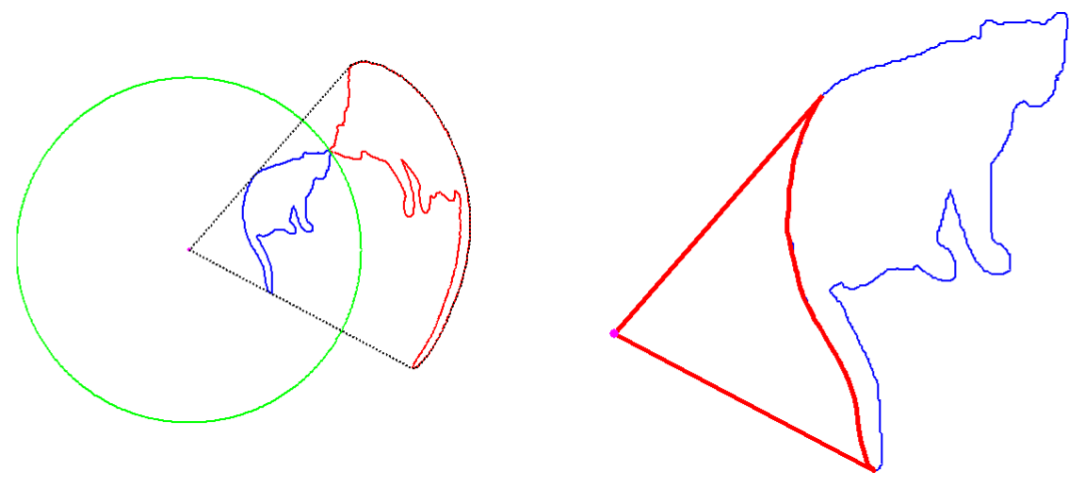
\includegraphics[width=7cm]{hpr.png}
	\end{center}
	\begin{enumerate}
	\item Center points around camera
	\item Spherical flipping transformation: \\
	$p' = p + 2(R - |p|) \frac{p}{|p|}$
	\item Compute convex hull (slow)
	\item Retain original points whose image is in c.h.
	\end{enumerate}
\end{frame}

\section{Data structures}

\begin{frame}{Data structures}
	\begin{itemize}
	\item Way to organize points
	\item Serialized into 1D memory
	\item $\rightarrow$ Using \emph{HDF5} file format
	\item Filtering implemented on top of data structure
	\item Prefer reading few long segments
	\item $\rightarrow$ Try to keep close points together in serialization
	\end{itemize}
\end{frame}

\begin{frame}{Cuboid regions}
	\begin{itemize}
	\item Technique: Subdivide into cuboid regions
	\item Downsampling ratio $r(d)$ per region
	\item $d$: \emph{point-to-cuboid} distance to camera
	\item $\rightarrow$ Need to choose compromise definition
	\end{itemize}
\end{frame}

\subsection{Cubes structure}

\begin{frame}{Cubes structure}
	\begin{itemize}
	\item Use grid of cubic regions
	\item Common side length
	\item Extract points from cubes that are inside frustum
	\item $\rightarrow$ Cuboid-frustum intersection test
	\item Both \emph{weighted points} and \emph{LOD regions} variants
	\end{itemize}
\end{frame}

\begin{frame}{Cubes structure (2)}
	\begin{center}
	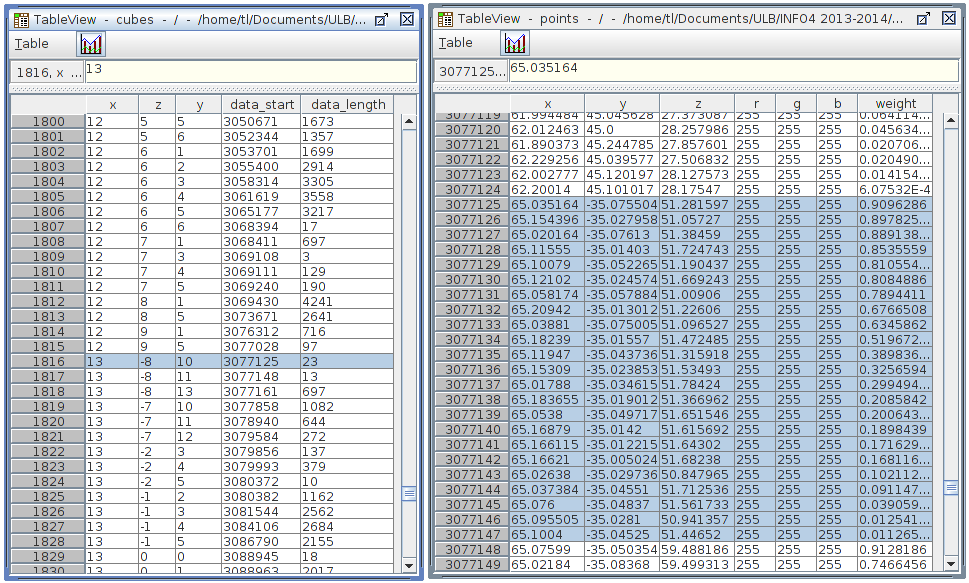
\includegraphics[width=\textwidth]{cubes_hdf.png} \\
	\end{center}
\end{frame}

\subsection{Tree structures}

\begin{frame}{Tree structures}
	\begin{columns}[c]
	\begin{column}[T]{.6\textwidth}
		\begin{itemize}
		\item Recursively subdivide
		\item ...until $\leq$ \emph{leaf capacity} points in cuboid
		\item Points in any node remain in one segment
		\item Can include/exclude large nodes
		\item $\rightarrow$ No need to test all leaves
		\item Variants: Octree, KdTree
		\end{itemize}
	\end{column}
	\begin{column}[T]{.4\textwidth}
		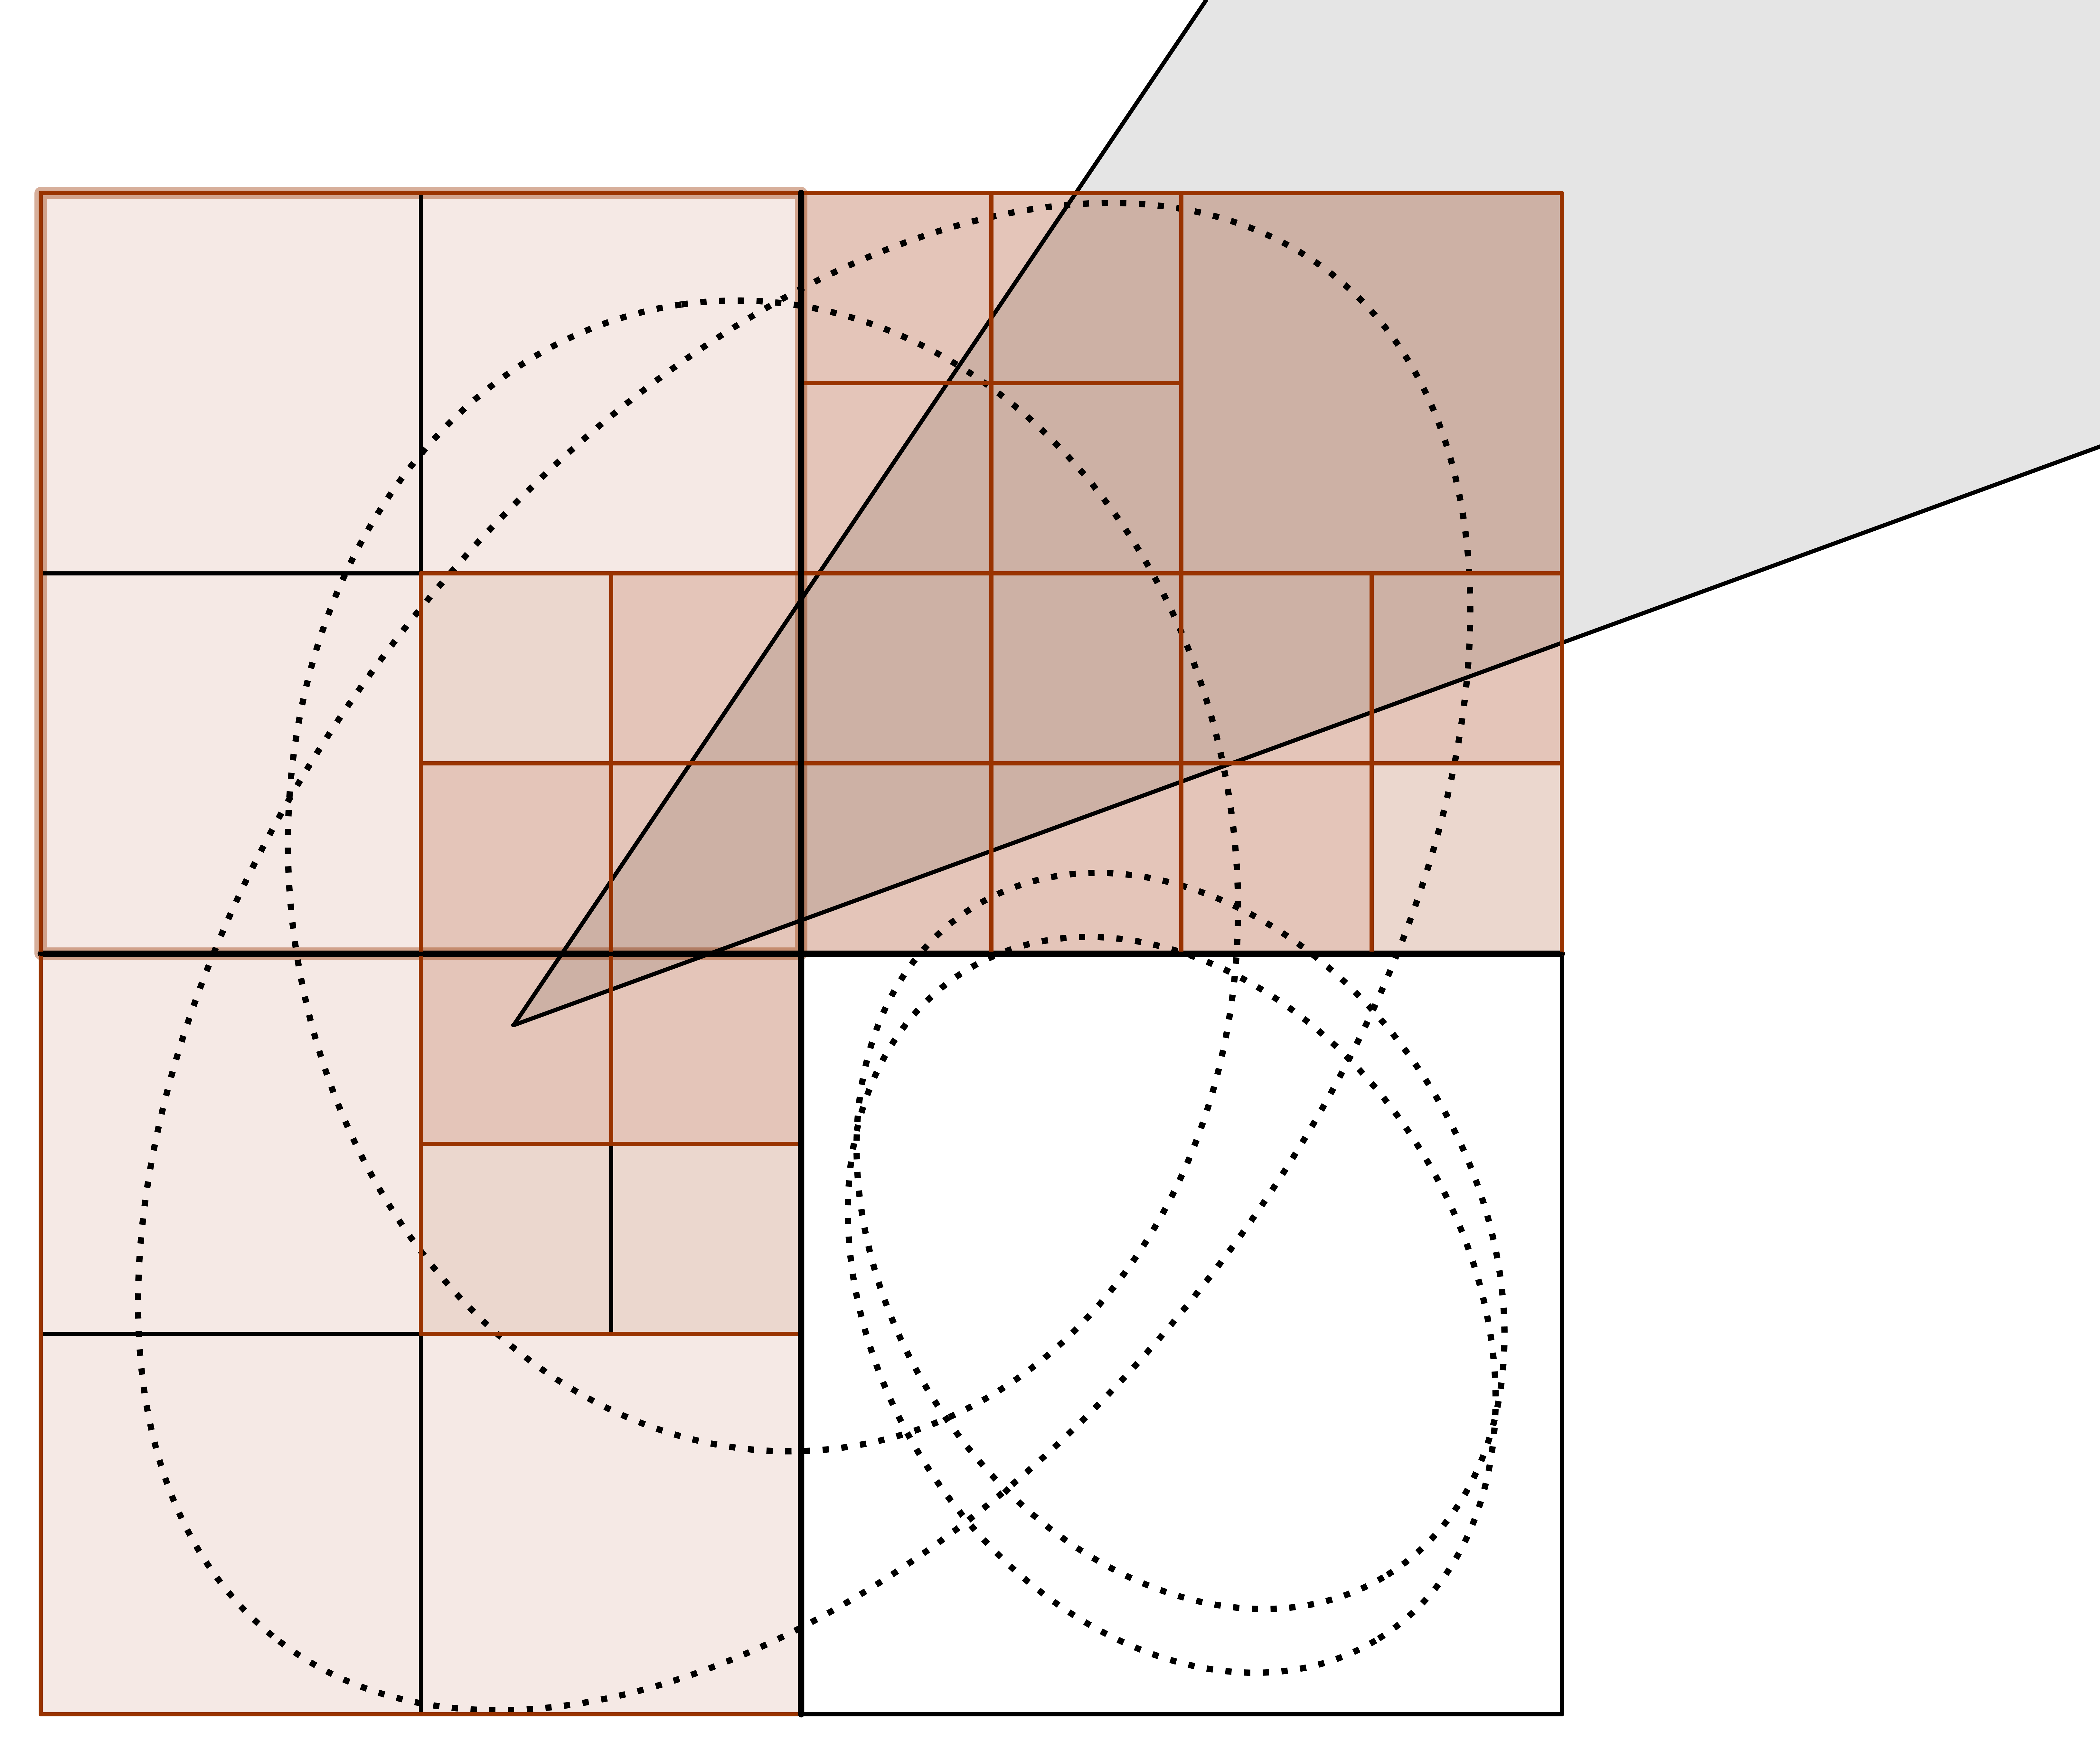
\includegraphics[width=4cm]{octree.png} \\
		Octree Example
	\end{column}
	\end{columns}
\end{frame}

\begin{frame}{Tree structures (2)}
	\begin{center}
	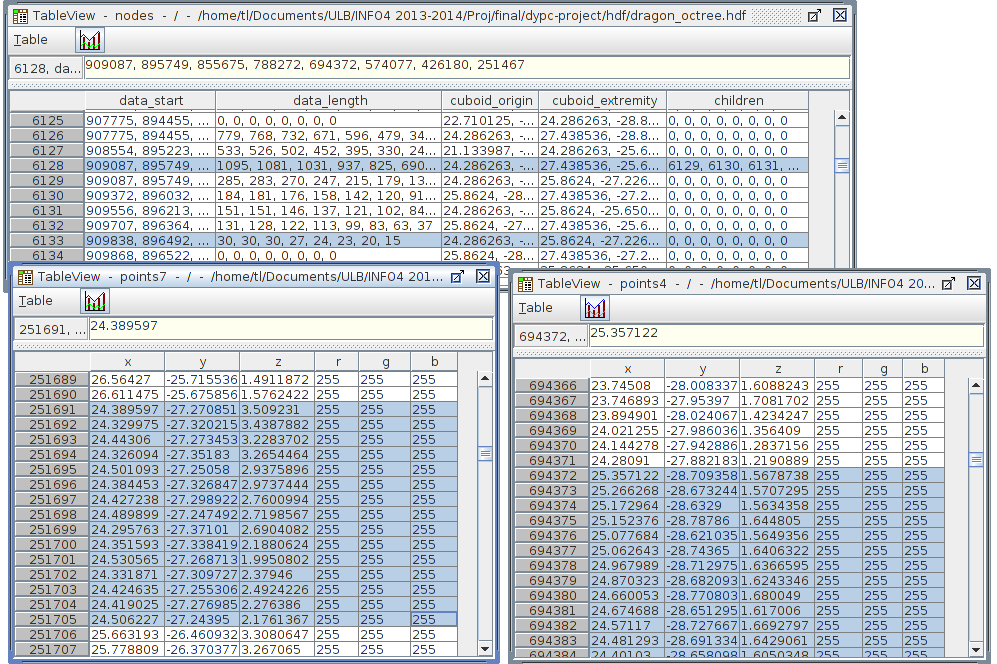
\includegraphics[width=\textwidth]{tree_hdf.png} \\
	\end{center}
\end{frame}

\begin{frame}{Octree}
	\begin{itemize}
	\item Regions always cubes
	\item Split into 8 child nodes
	\end{itemize}
	\begin{center}
	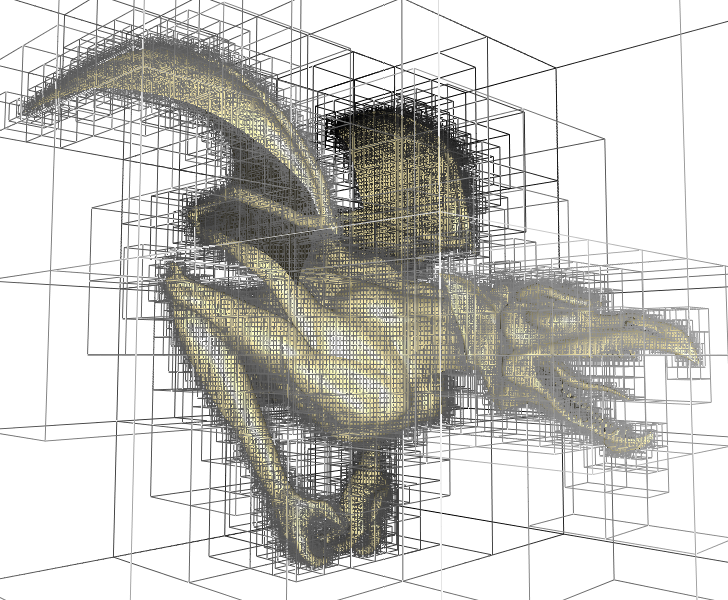
\includegraphics[width=.7\textwidth]{octree_dragon.png} \\
	\end{center}
\end{frame}

\begin{frame}{Octree}
	\begin{itemize}
	\item Split into 2 child nodes
	\item Split plane = median
	\item $\Rightarrow$ balanced tree
	\item in X, Y, Z, X... axis (depth modulo 3)
	\end{itemize}
	\begin{center}
	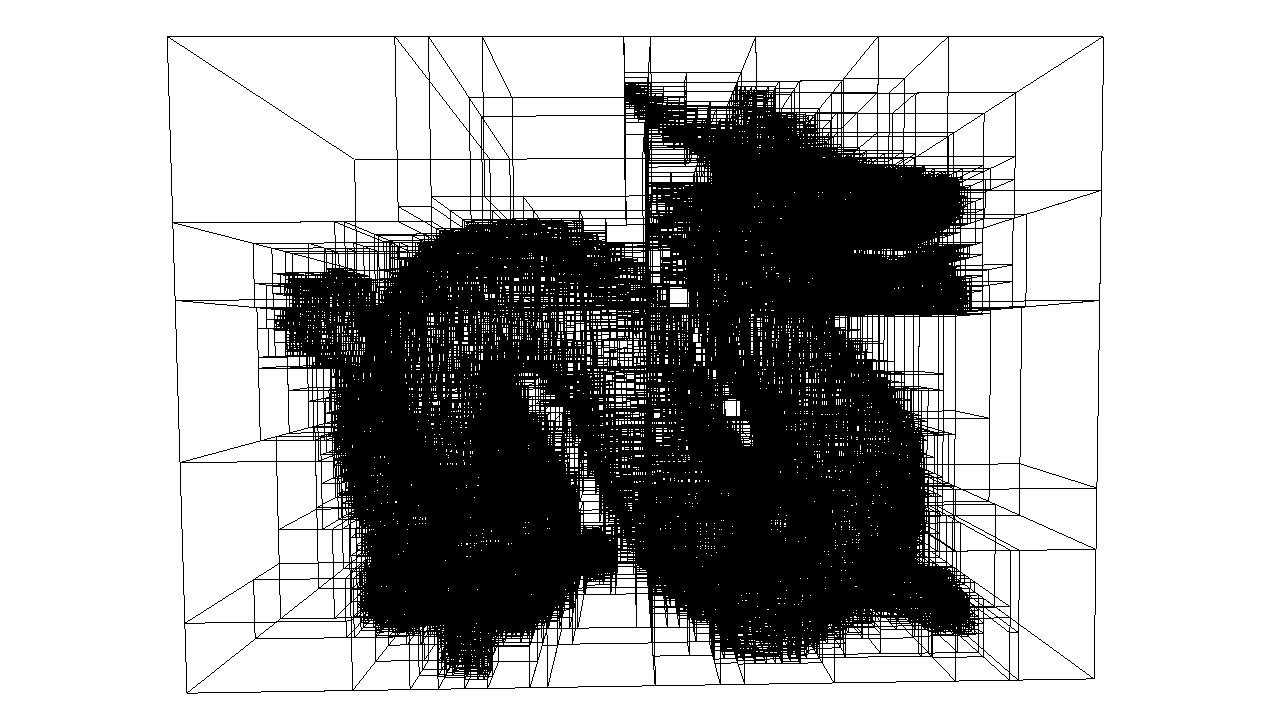
\includegraphics[width=.8\textwidth]{kdtree_dragon.jpg} \\
	\end{center}
\end{frame}

\subsection{Piecewise construction}

\begin{frame}{Piecewise construction}
	\begin{itemize}
	\item One \emph{Outer tree} without points
	\item Several \emph{inner trees} at leaves of outer tree
	\item Different tree types possible
	\item $\rightarrow$ KdTree-Median good for outer tree
	\item Load one+ inner tree at a time
	\item $\rightarrow$ Limit memory usage
	\item $\rightarrow$ Parallization possible
	\end{itemize}
\end{frame}

\section{Implementation}

\begin{frame}{Implementation}
	\begin{description}
	\item[libdypc.so] Library containing all algorithms / structures
	\item[viewer] GUI front-end and dynamic renderer
	\end{description}
	Implemented in C++ \\
	Pure C library API interface
\end{frame}

\begin{frame}{Streaming Mechanism}
	\begin{itemize}
	\item 2 threads
		\begin{description}
		\item[renderer] main GUI, renders from point buffer
		\item[loader] periodically extracts new point set
		\end{description}
	\item Update via OpenGL buffer swap
	\item $\rightarrow$ Loader writes directly into GPU buffer
	\item Update when camera position/orientation changes
	\end{itemize}
\end{frame}

\end{document}
